
%%% Local Variables: 
%%% mode: latex
%%% TeX-master: t
%%% End: 

\chapter{模块实现}

每个模块对应了一类题型,即一个Activity和其对应的Question。在这次设计中,充分运用了Android的界面设计(即每个Activity可以对应一个XML文件),这样可以加速程序加载,也可以通过界面中组件的ID进行个性化设置。

\section{登陆模块}

\begin{figure}[h]
\centering%
\begin{subfigure}{6cm}
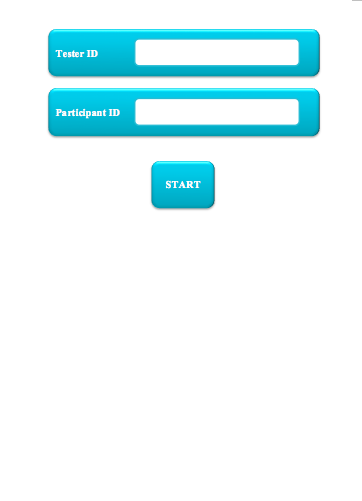
\includegraphics[width=6cm]{loginD}
\caption{登陆模块-设计}
\end{subfigure}
\hspace{4em}%
\begin{subfigure}{6cm}
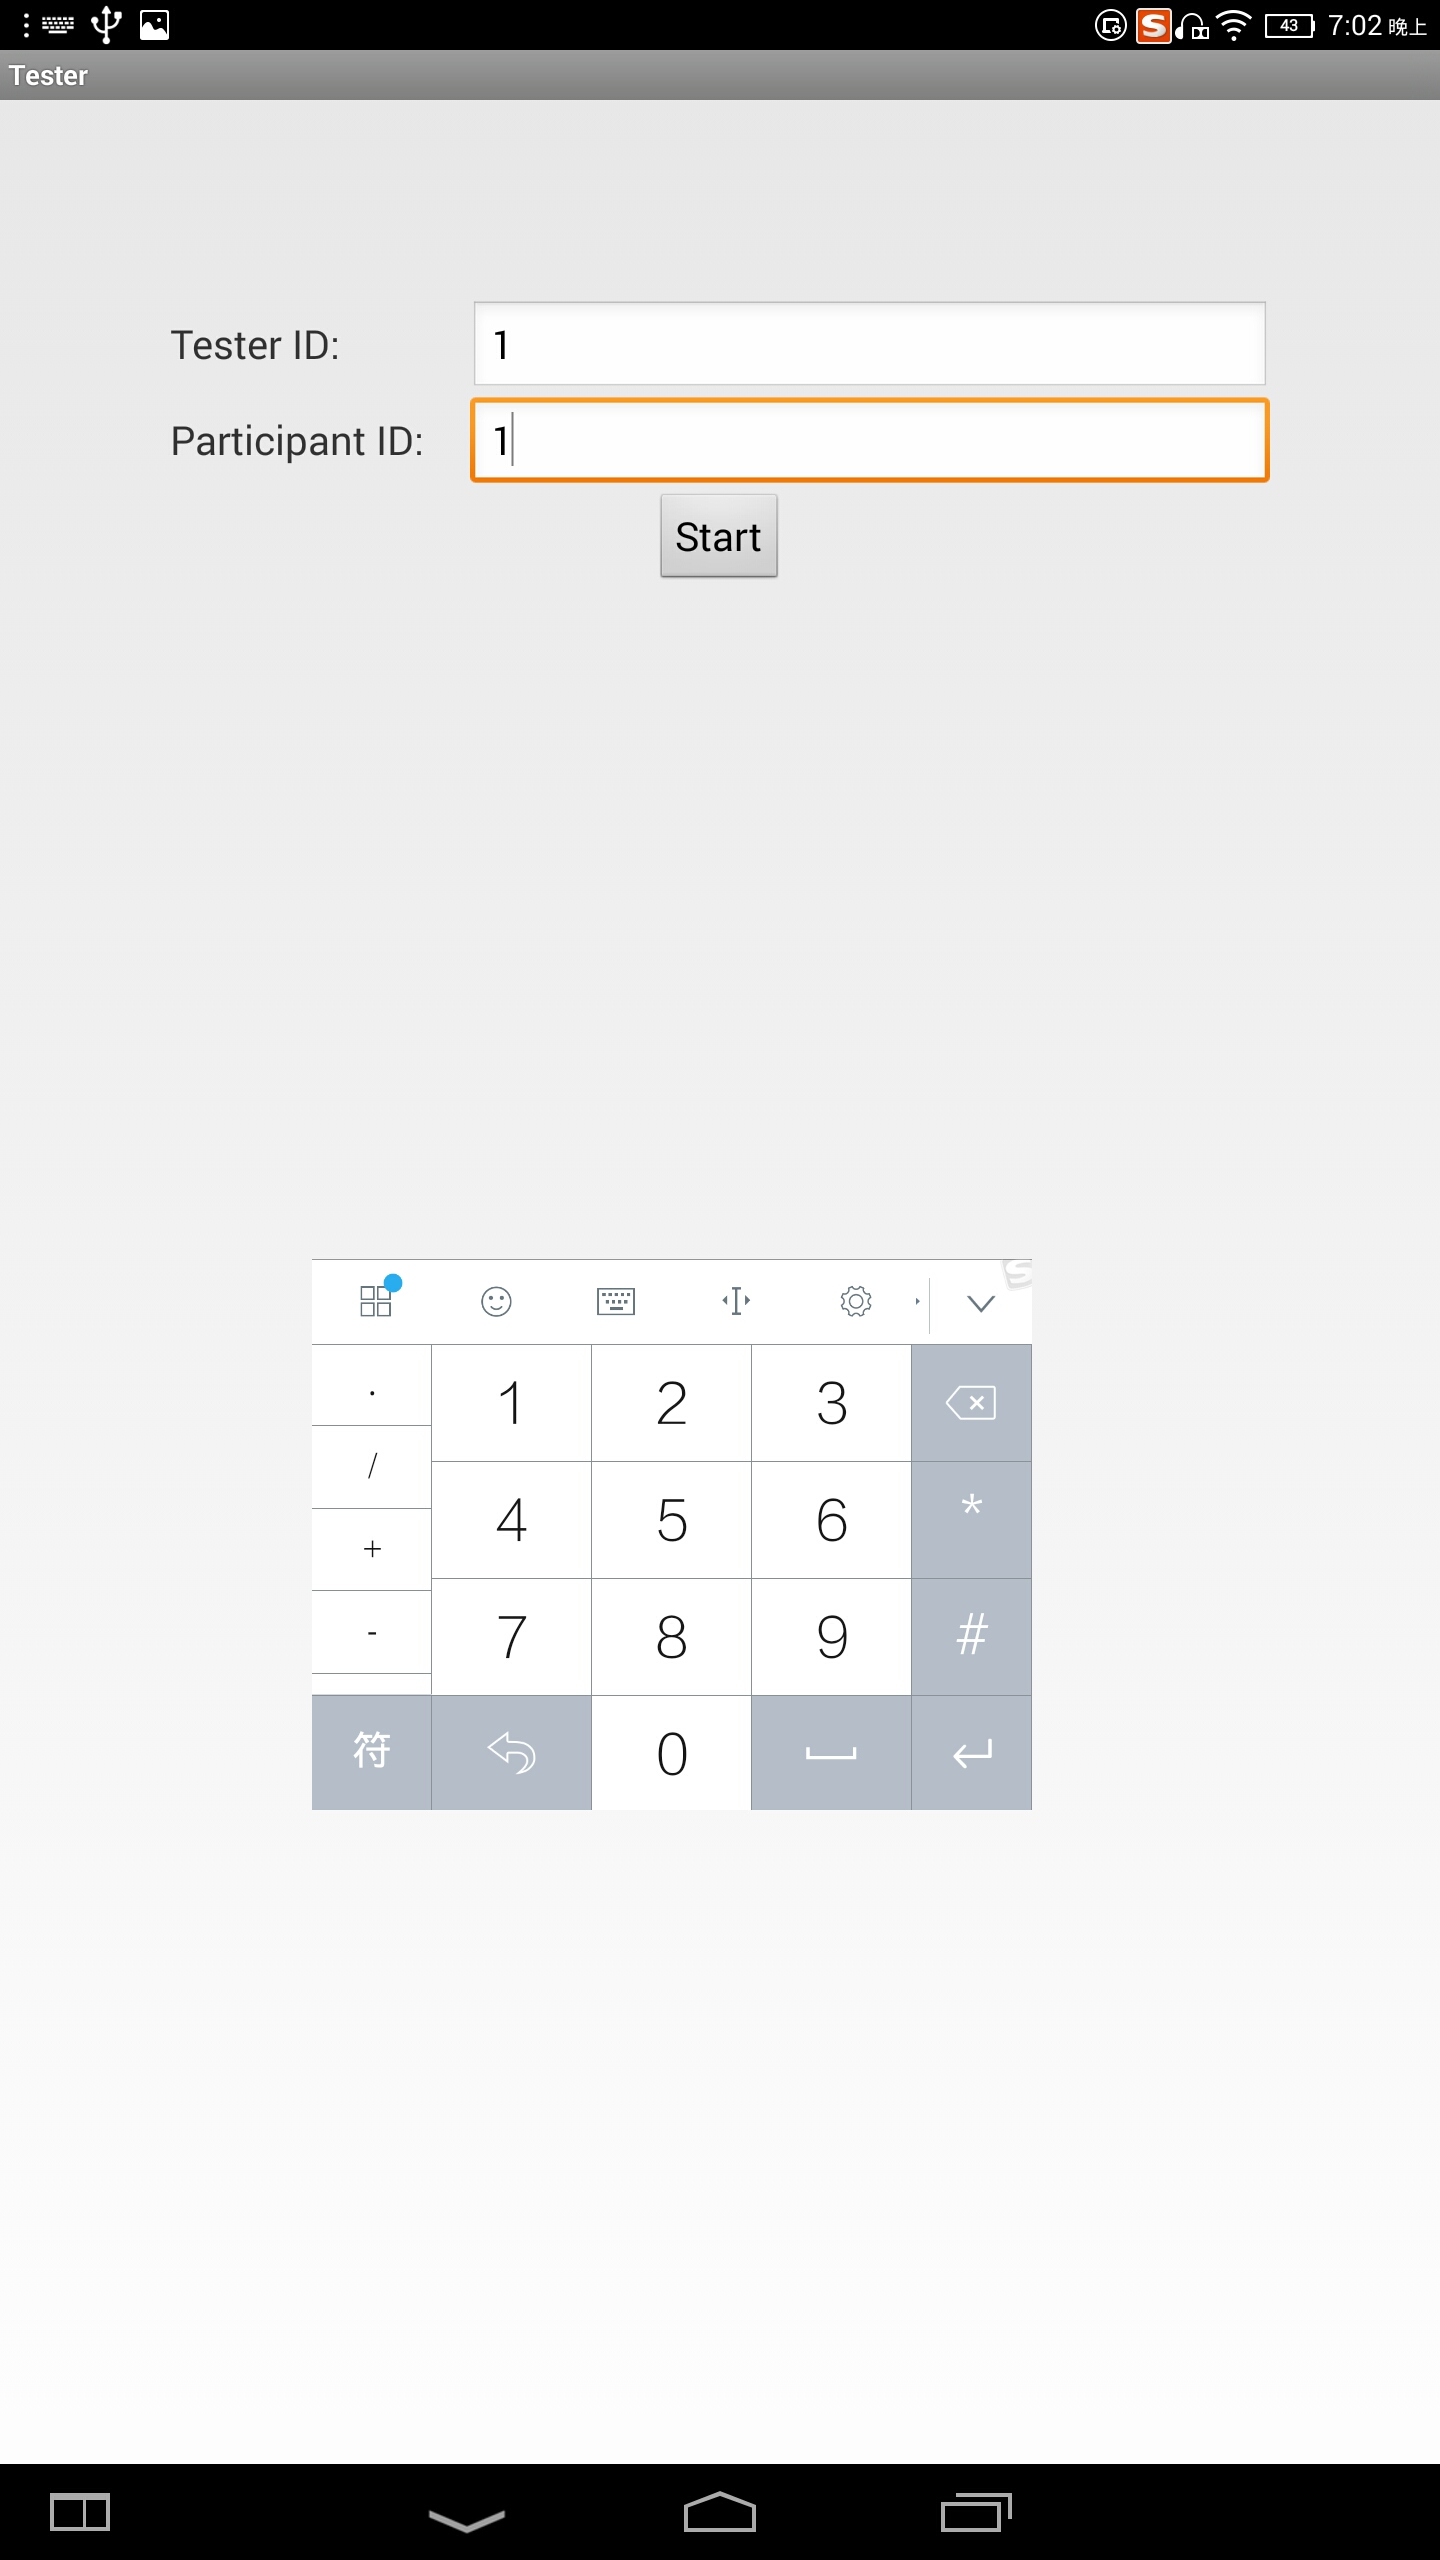
\includegraphics[width=6cm]{login}
\caption{登陆模块-最终实现}
\end{subfigure}
\caption{登陆模块设计和最终实现图}
\label{fig:big1-subfigure}
\end{figure}

登陆模块是整个APP的开始,三个版本的APP中都会包括这个模块,在这个模块中会对程序所有需要的配置和变量进行初始化(所有的题目以及需要评分的答案)。而这个模块的主要功能为确定医生ID和病人ID设计,这样可以使测试得到的数据与日期、病人一一对应,其中在数据库中已经建立了匹配的字符串对(储存在OSS平台上的配置文件目录下的IDmap.txt里),生成规则由波士顿大学给出。该模块的逻辑比较简单,即获取界面上用户输入的TesterID和ParticipanterID后连接数据库,与数据库中的配对进行匹配即可,若成功,则进入第一题,否则弹出一个错误提示对话框,说明数据库中没有对应匹配,要求用户重新输入再次尝试。

\section{故事复述题模块}

\begin{figure}[h]
\centering%
\begin{subfigure}{6cm}
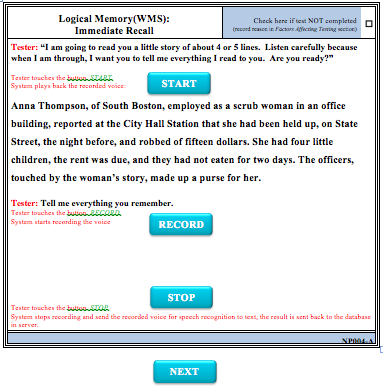
\includegraphics[width=6cm]{storyD}
\caption{数字串复述题-设计}
\end{subfigure}
\hspace{4em}%
\begin{subfigure}{6cm}
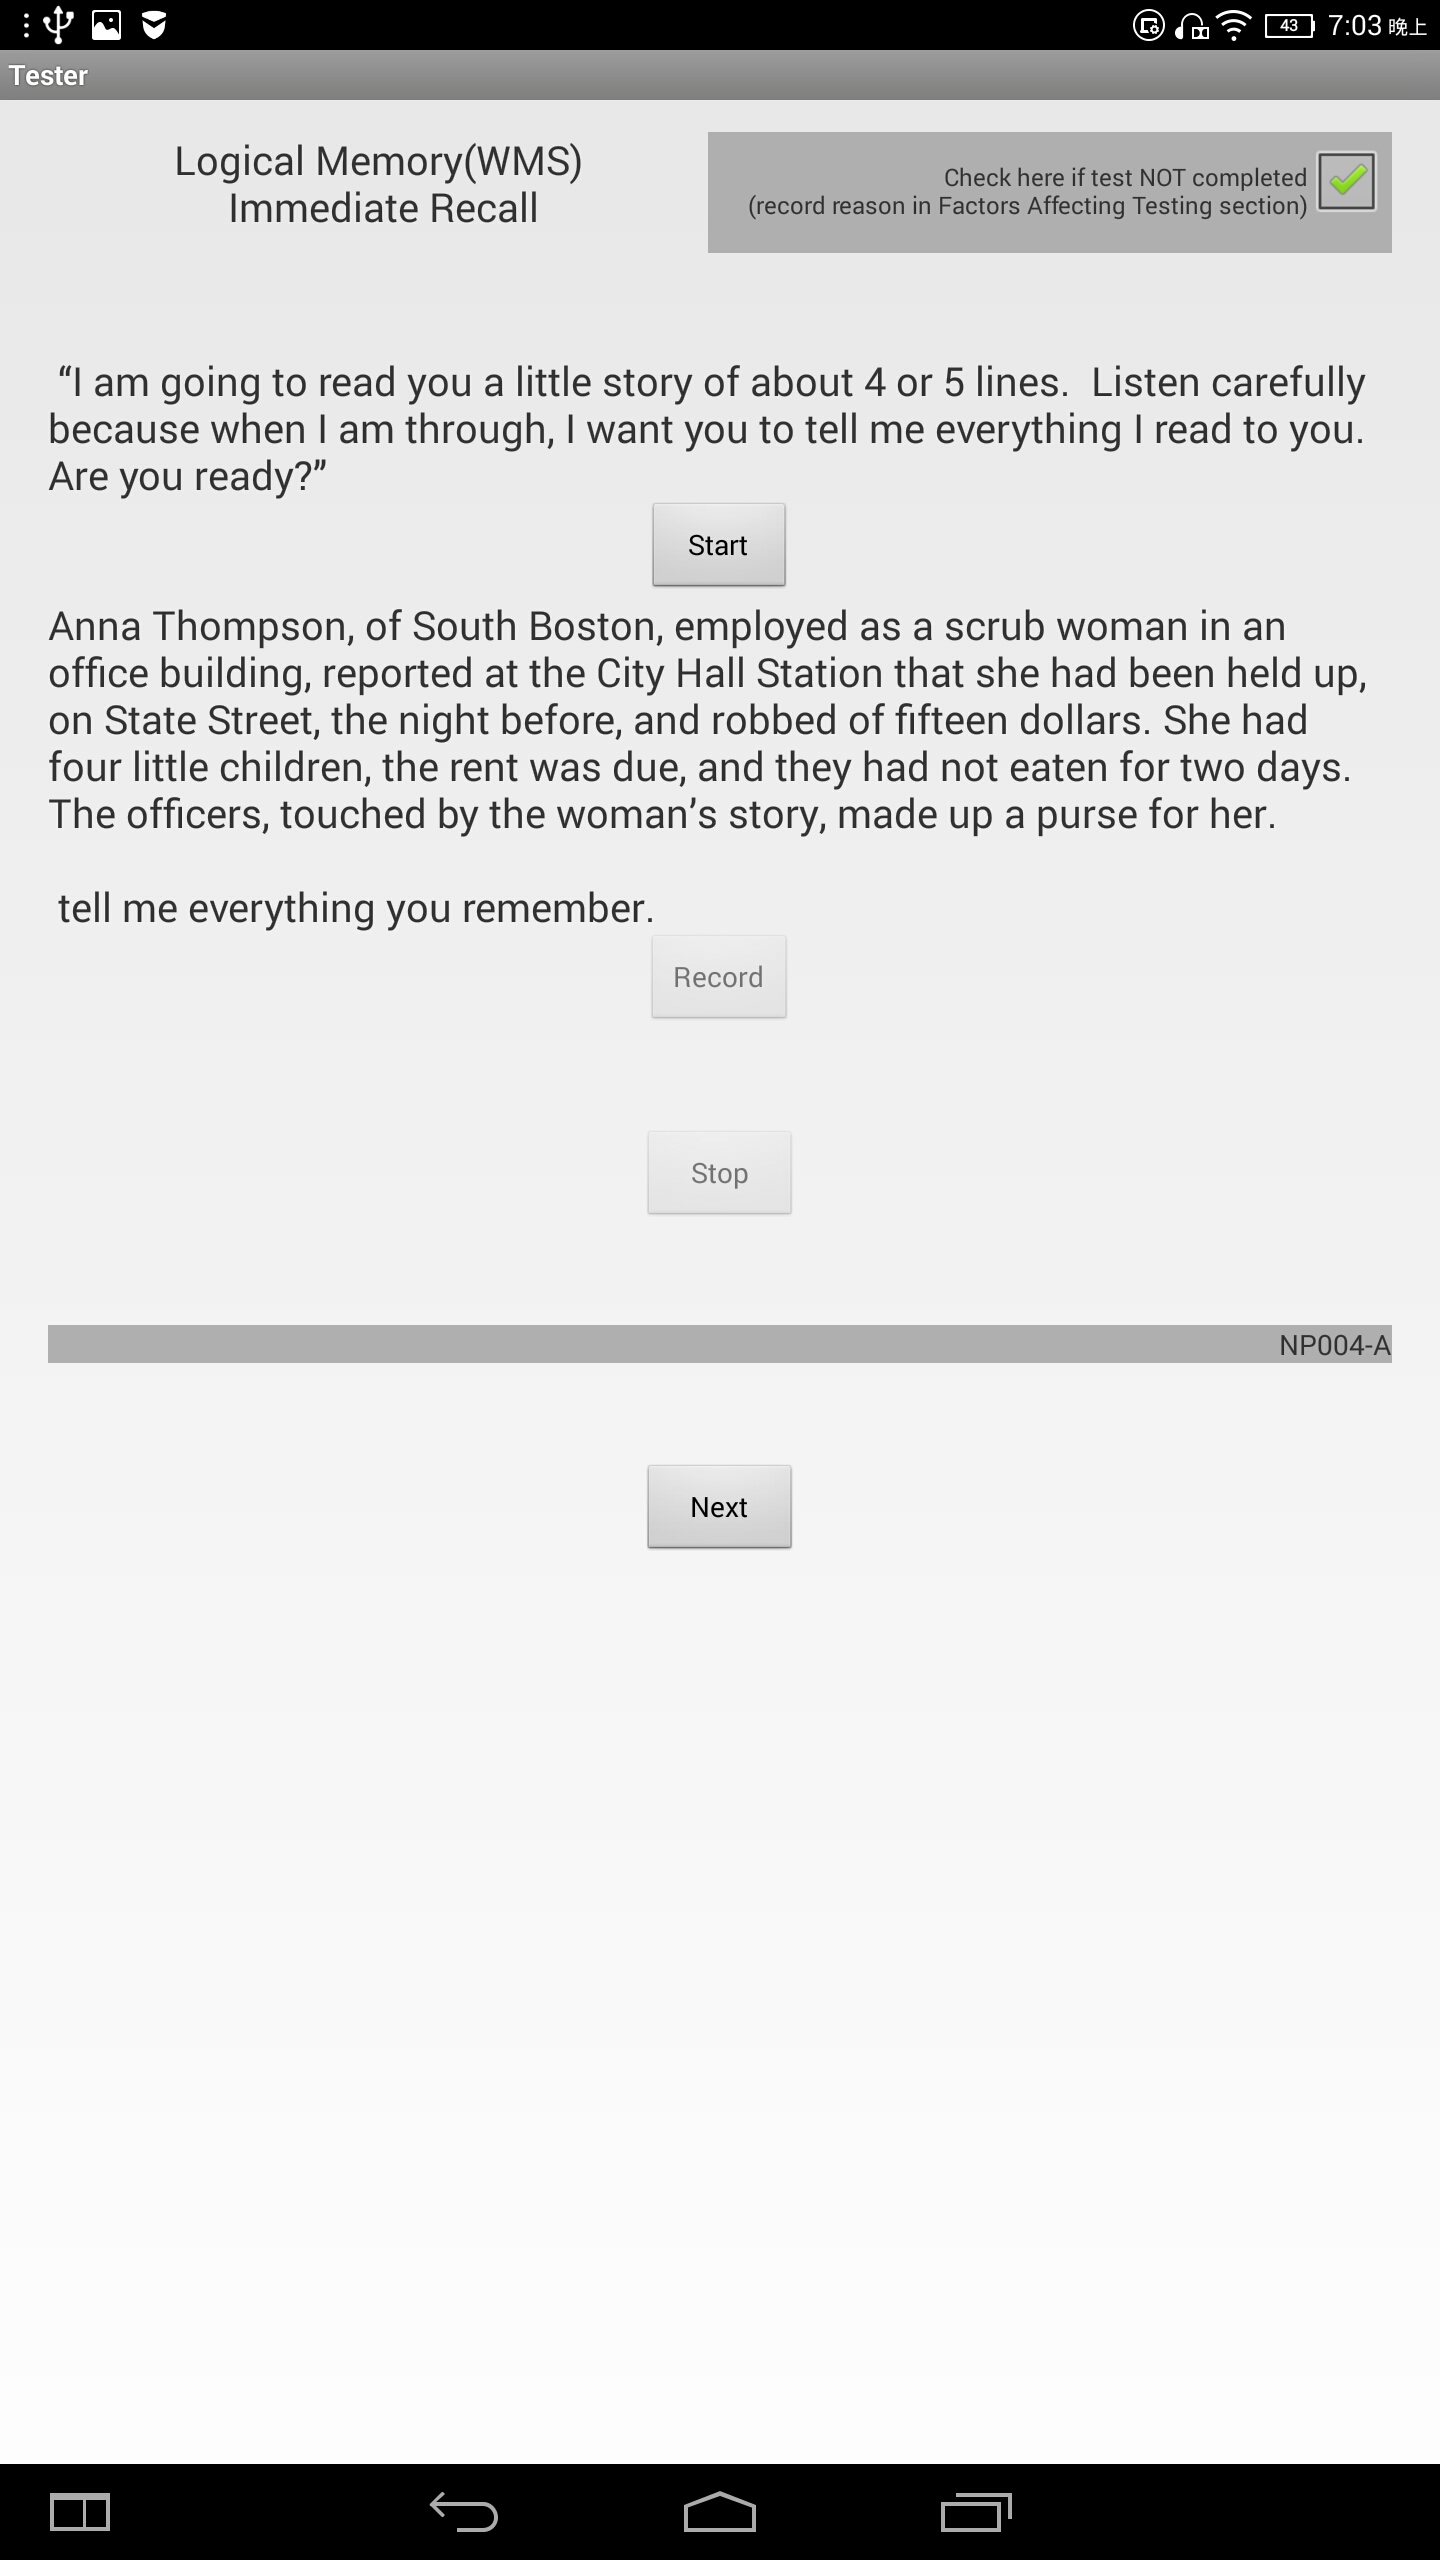
\includegraphics[width=6cm]{story}
\caption{故事复述题-最终实现}
\end{subfigure}
\caption{故事复述题设计和最终实现图}
\label{fig:big1-subfigure}
\end{figure}

故事复述题包括在线测试版和离线打分版两部分。对于在线测试版,除了界面上需要有提示词之外,需要有播放录音、以及音频录制的功能。这里直接使用了Android自带的MediaPlayer和MediaRecorder,根据题目JSON中的信息,查找已经放在工程中对应的音频文件,点击Start按钮后进行播放;同样也根据JSON中录音名的信息,在平板电脑的根目录下创建对应的临时文件,并在用户点击下一题时上传该文件,然后删除这个临时文件。这里为了引导用户按照顺序(播放录音、录制、停止录制),为按钮设置了可按的顺序(即开始只能播放录音、在播放完录音后才能开始录制音频,在开始录音后才能选择停止录制)。

\begin{figure}[h]
\centering%
\begin{subfigure}{6cm}
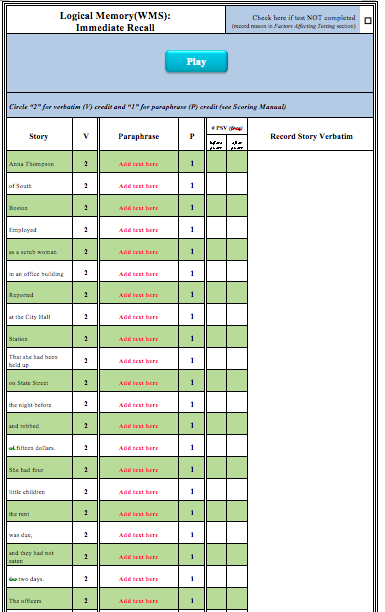
\includegraphics[width=6cm]{storyscoreD}
\caption{数字串复述题离线打分版-设计}
\end{subfigure}
\hspace{4em}%
\begin{subfigure}{6cm}
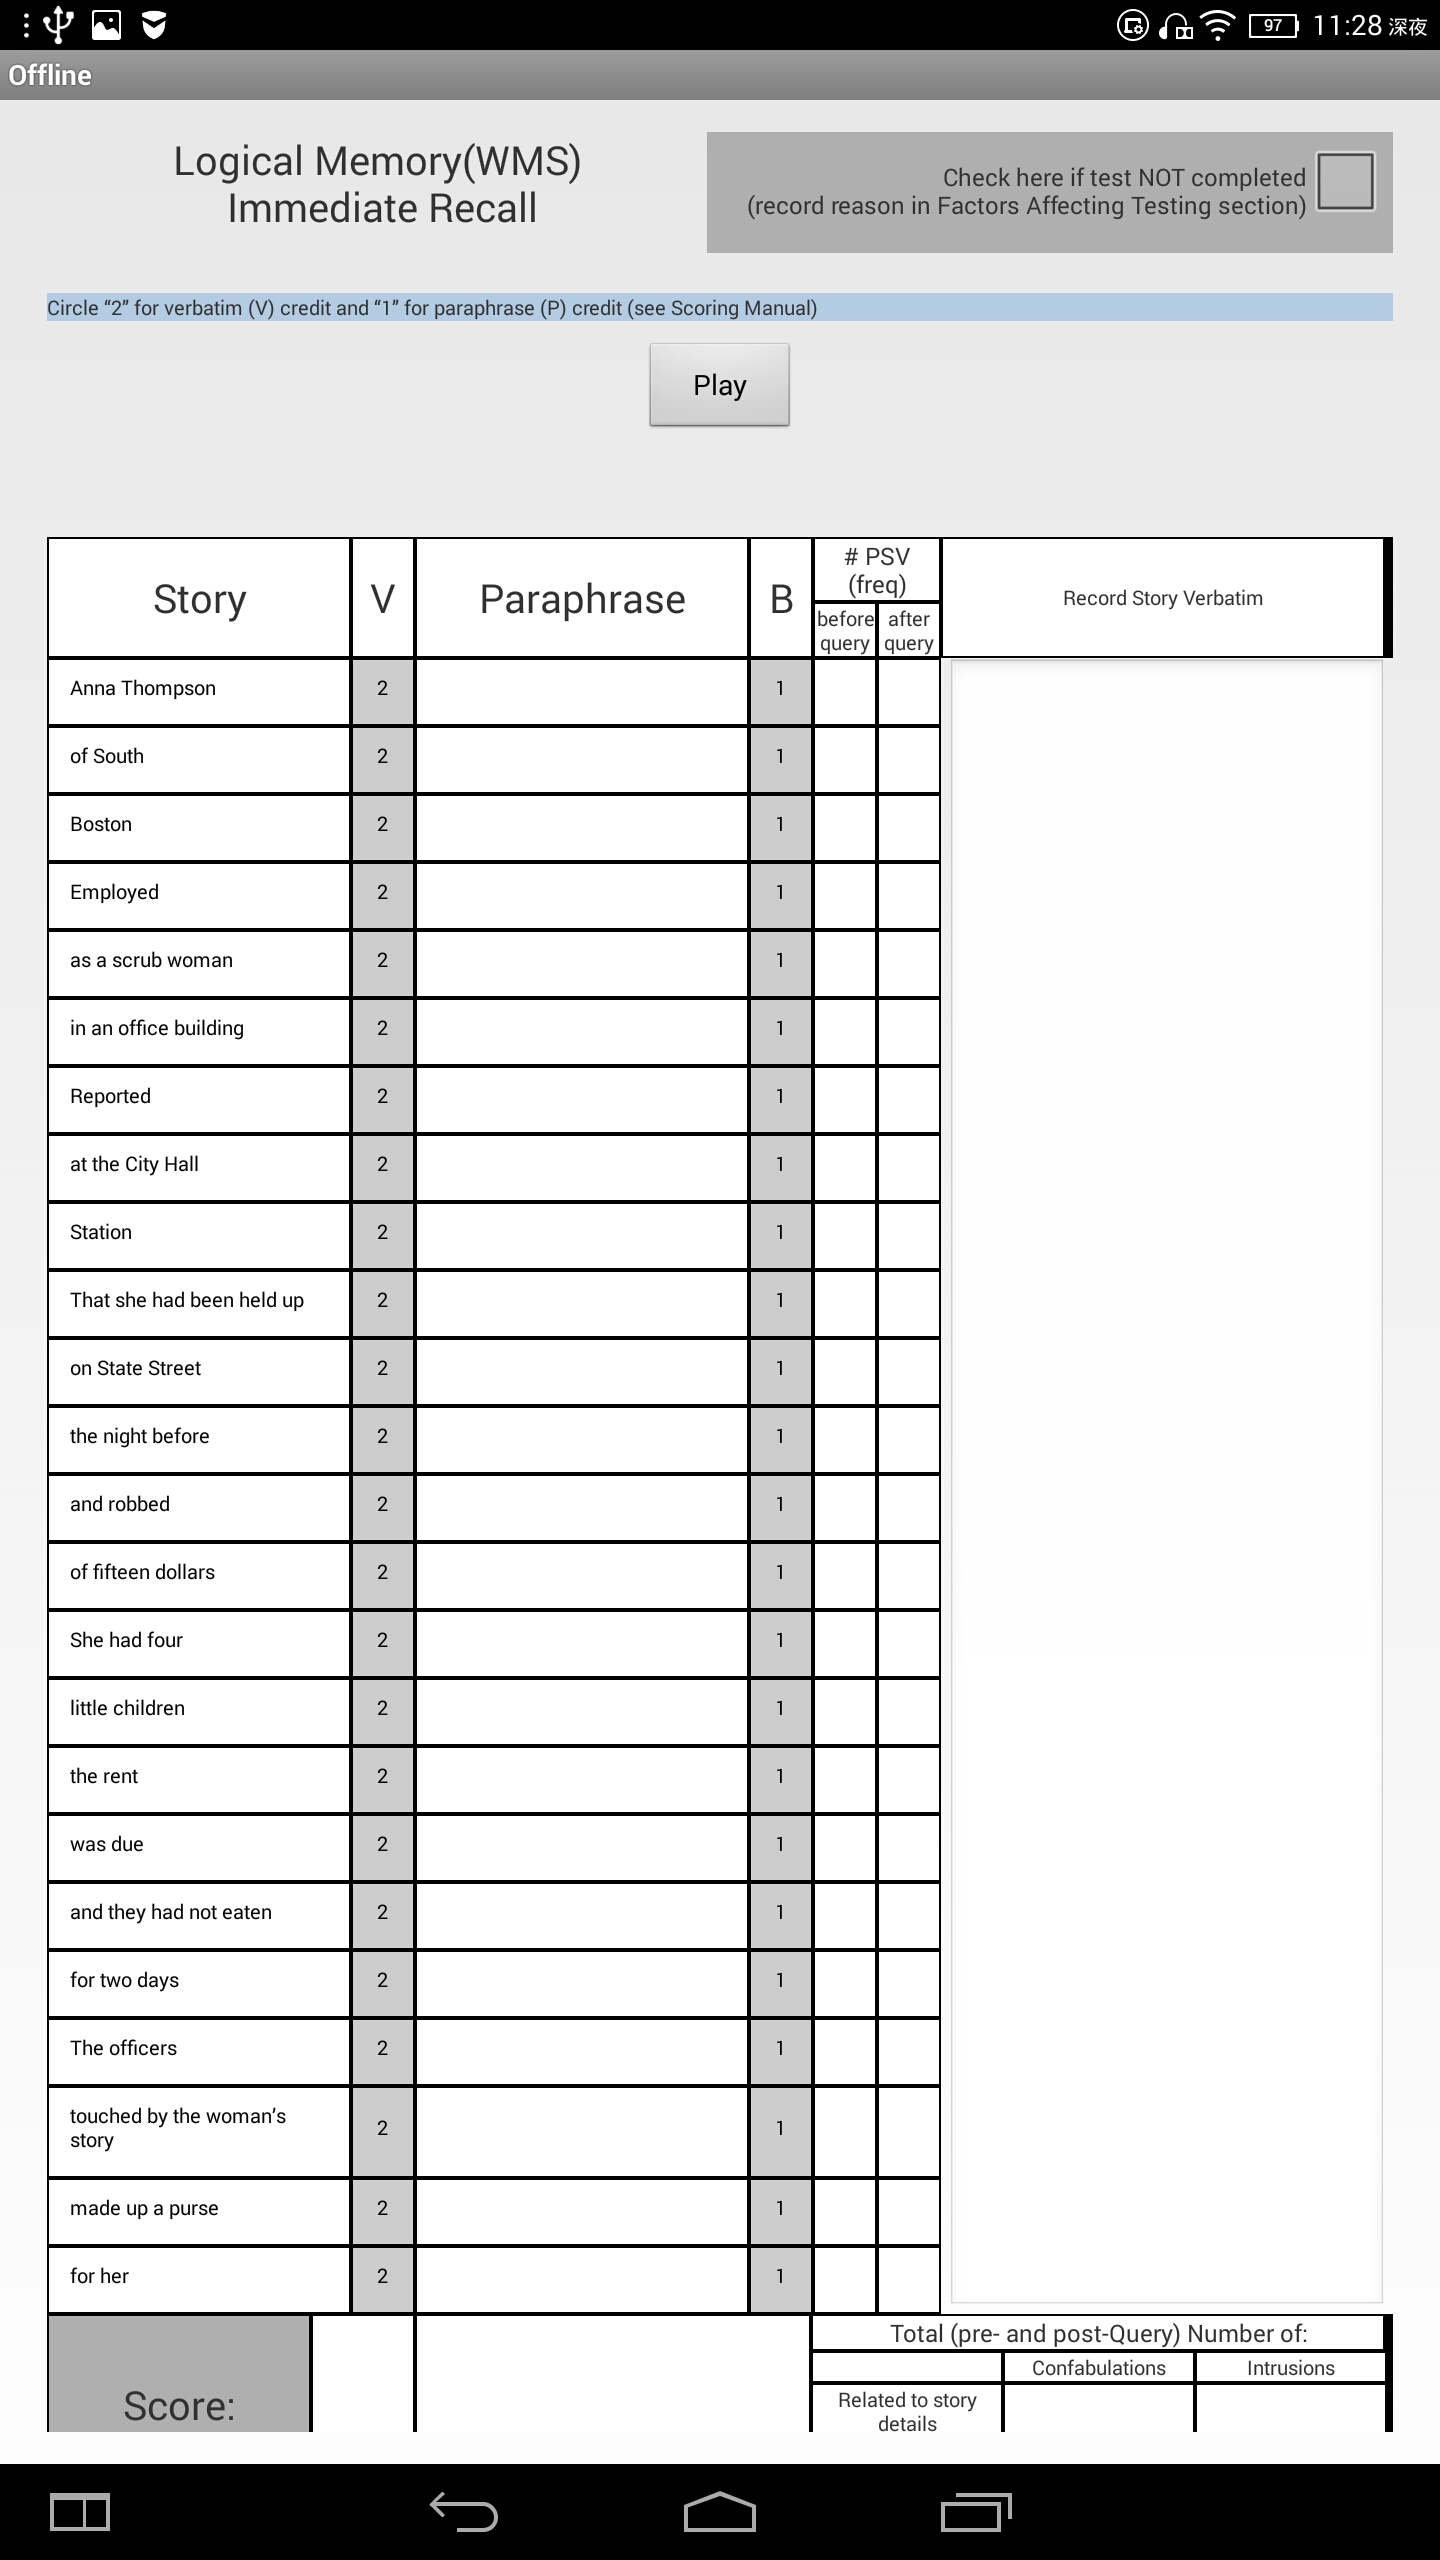
\includegraphics[width=6cm]{storyscore}
\caption{故事复述题离线打分版-最终实现}
\end{subfigure}
\caption{故事复述题离线打分版设计和最终实现图}
\label{fig:big1-subfigure}
\end{figure}

离线打分版需要展示所有打分项,以及播放录音、识别录音信息等功能。在界面加载时,会根据题目JSON文件从OSS将需要的媒体文件下载(播放的录音),而题目的答案在初始APP已经更新。打分项的每一行都用自定义的SingleStoryScoreView作为界面组件,这个组件包括了故事、打分按钮和打分方框,独立定义组件是为了避免过多重复代码的写入。在计算分数时,会统计每个SingleStoryScoreView的得分再总和。播放录音同样使用Android自带的MediaPlayer。录音识别使用了百度语音识别的接口(在上一章的内容中已经介绍),通过监听回调结果并显示在界面,辅助用户快速做评分。

\section{画图题模块}

\begin{figure}[h]
\centering%
\begin{subfigure}{6cm}
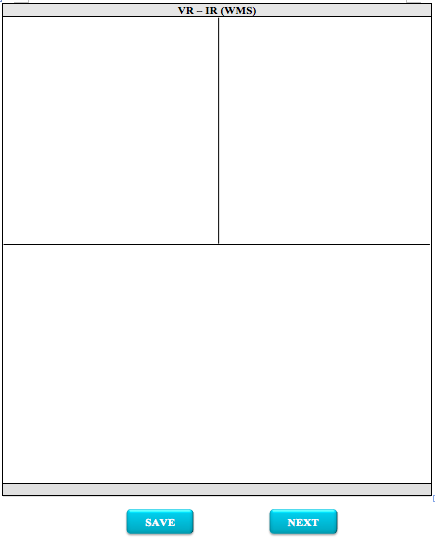
\includegraphics[width=6cm]{drawD}
\caption{画图题病人版-设计}
\end{subfigure}
\hspace{4em}%
\begin{subfigure}{6cm}
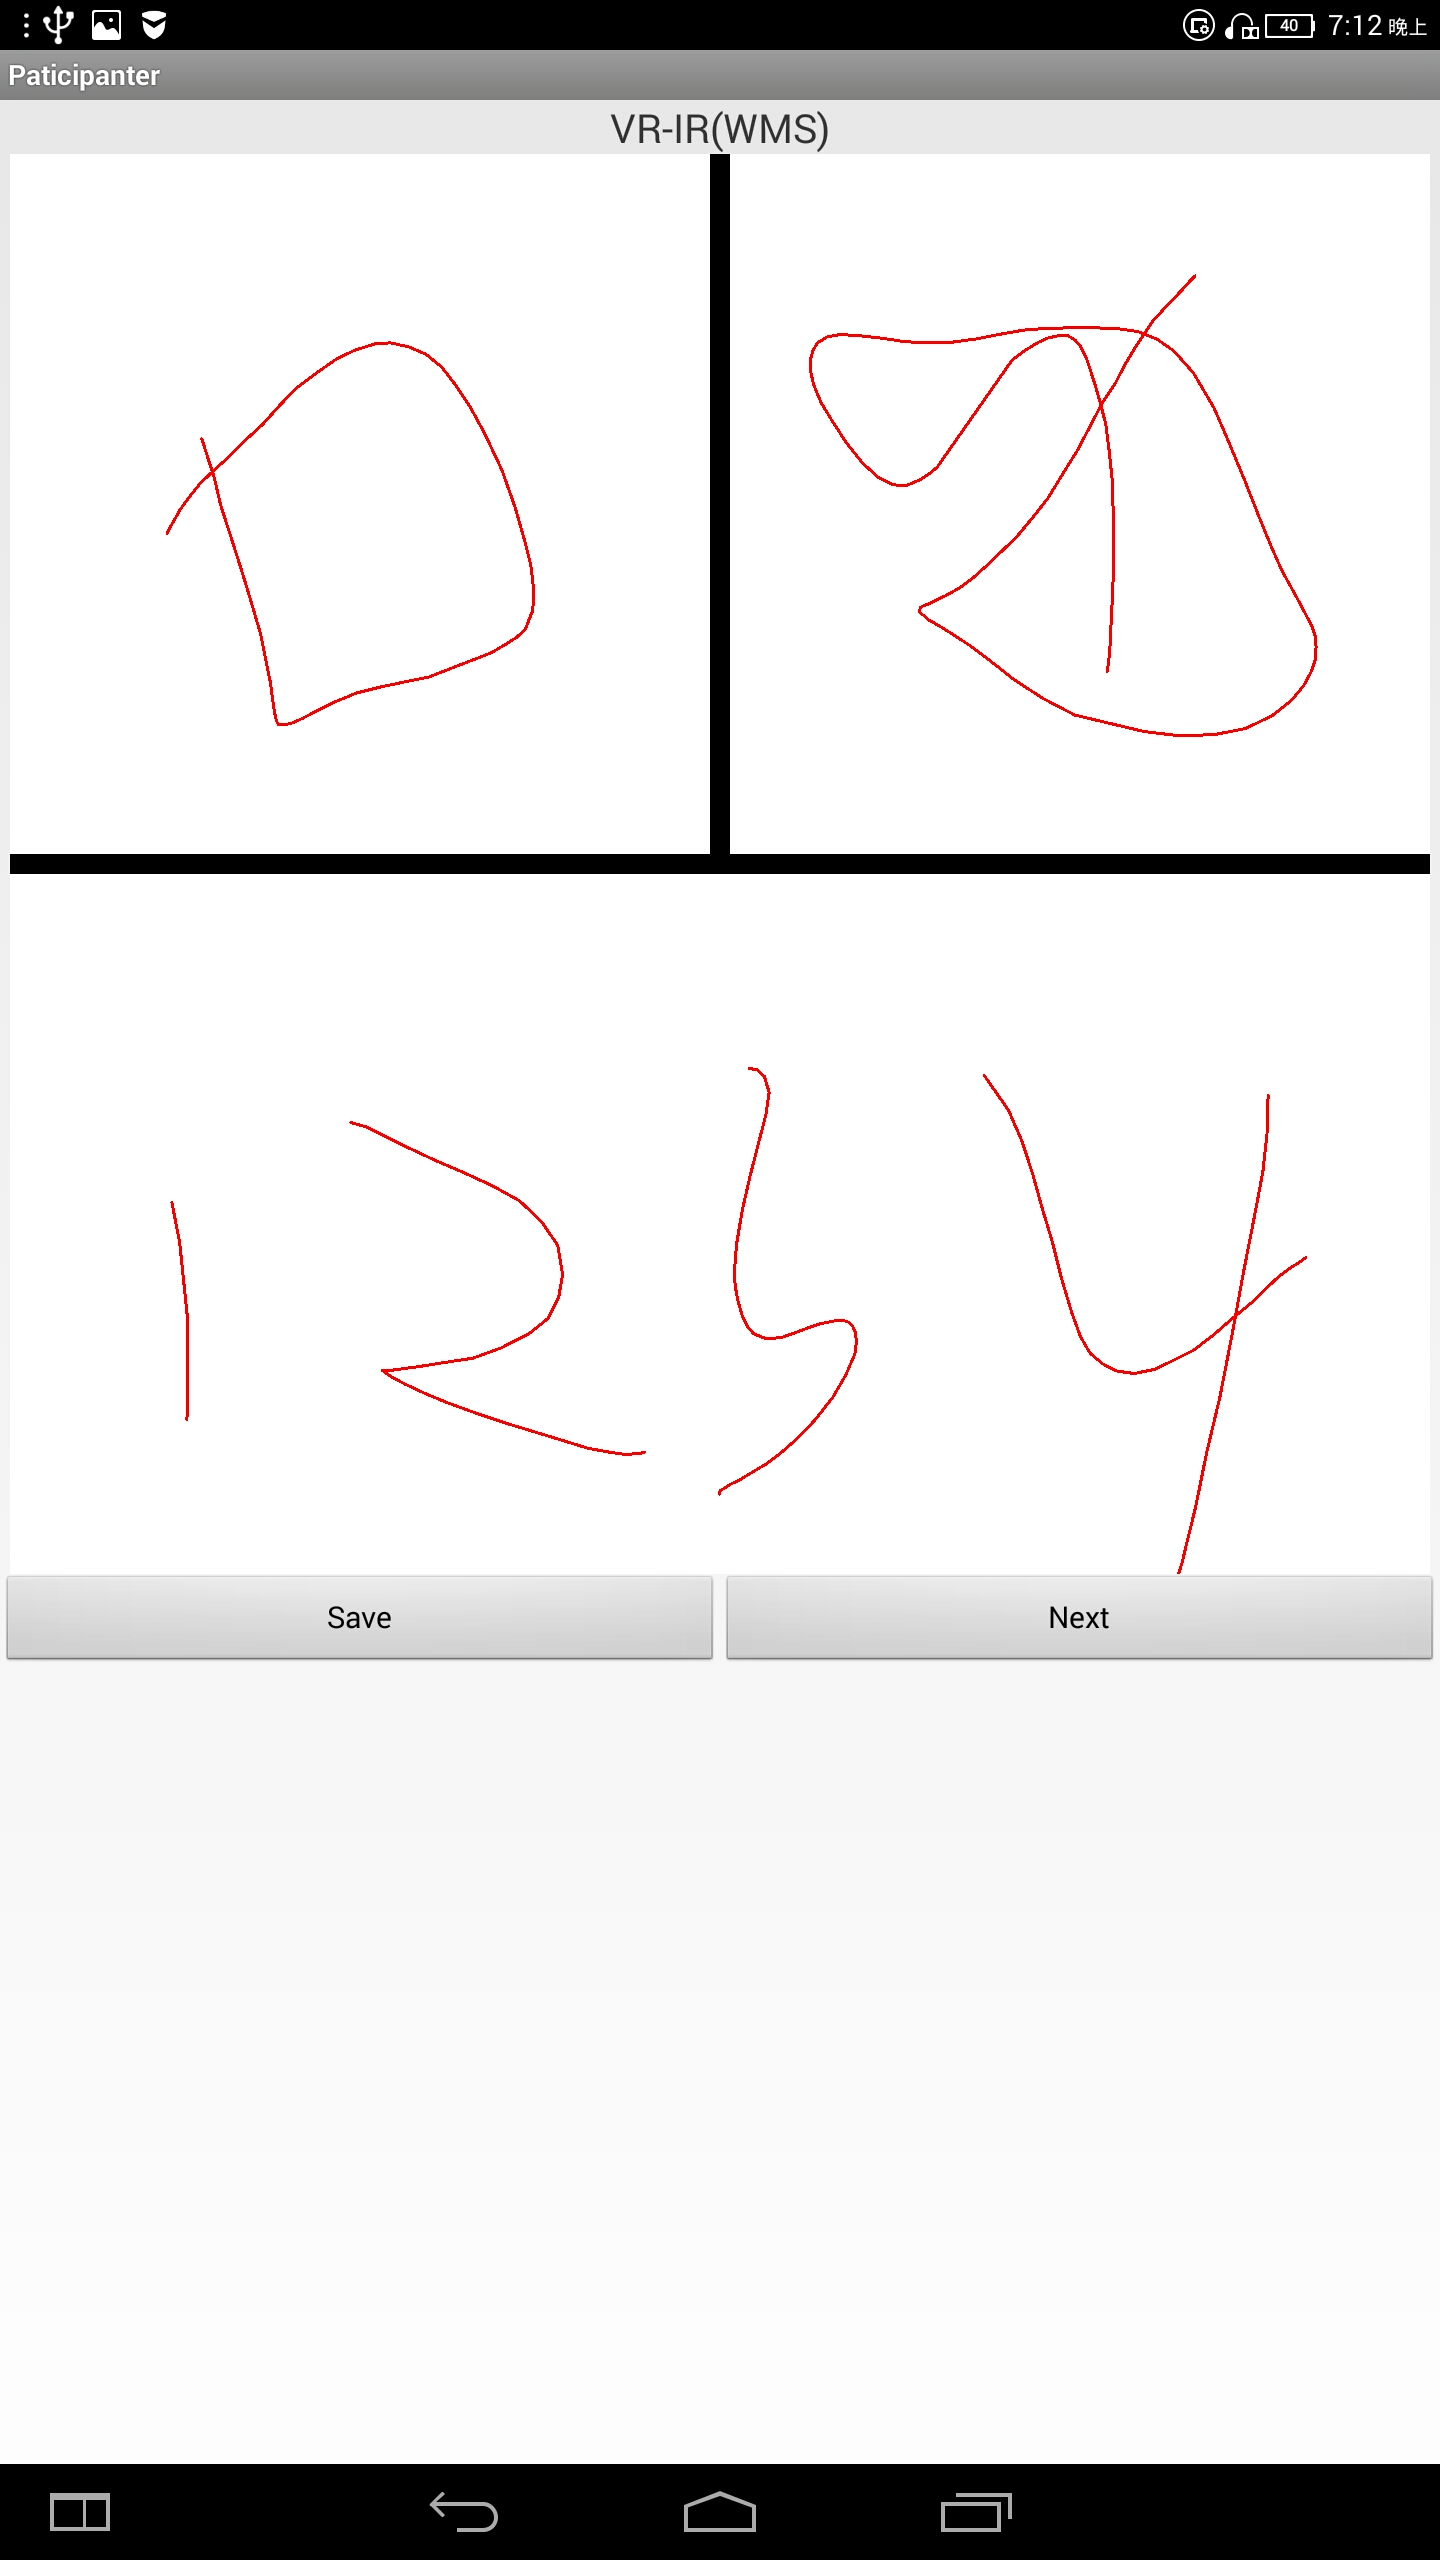
\includegraphics[width=6cm]{draw}
\caption{画图题病人版-最终实现}
\end{subfigure}
\caption{画图题设计和最终实现图}
\label{fig:big1-subfigure}
\end{figure}

画图题包括了在线病人版、在线医生版和离线打分版三个部分。为了还原和纸板一样的用户体验(即医生和用户都需要有“平板”在面前),在在线病人版和在线医生版中都存在。病人版主要是为了让病人能够画图,并能够记录下病人画图的轨迹。由于有些题目是有顺序的,这里也加入了顺序的概念,即界面上只有一处是可以画的,只有当病人点击“下一个”时,接下来需要画的部分才会打开。绘画过程主要用了Android自带的Paint工具,开启绘画的线程接收用户的点击并描绘和记录轨迹,在平板电脑的根目录下创建与题目JSON对应的临时文件,然后根据用户的选择进行上传。

在线医生版主要的功能是能够展示题目提示和限时展示图片,在展示图片时需要做到屏幕上只有图片而没有其他东西。这里的模块设计也完全按照顺序,根据用户的点击开启Handler计时、显示图片并隐藏其他内容,当Handler显示时间已经到时再恢复显示其他内容。

\begin{figure}[h]
\centering%
\begin{subfigure}{6cm}
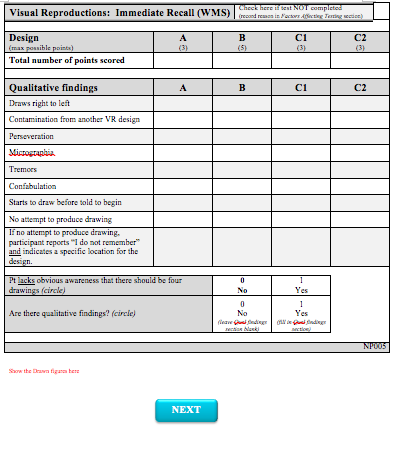
\includegraphics[width=6cm]{drawscoreD}
\caption{画图题离线打分版-设计}
\end{subfigure}
\hspace{4em}%
\begin{subfigure}{6cm}
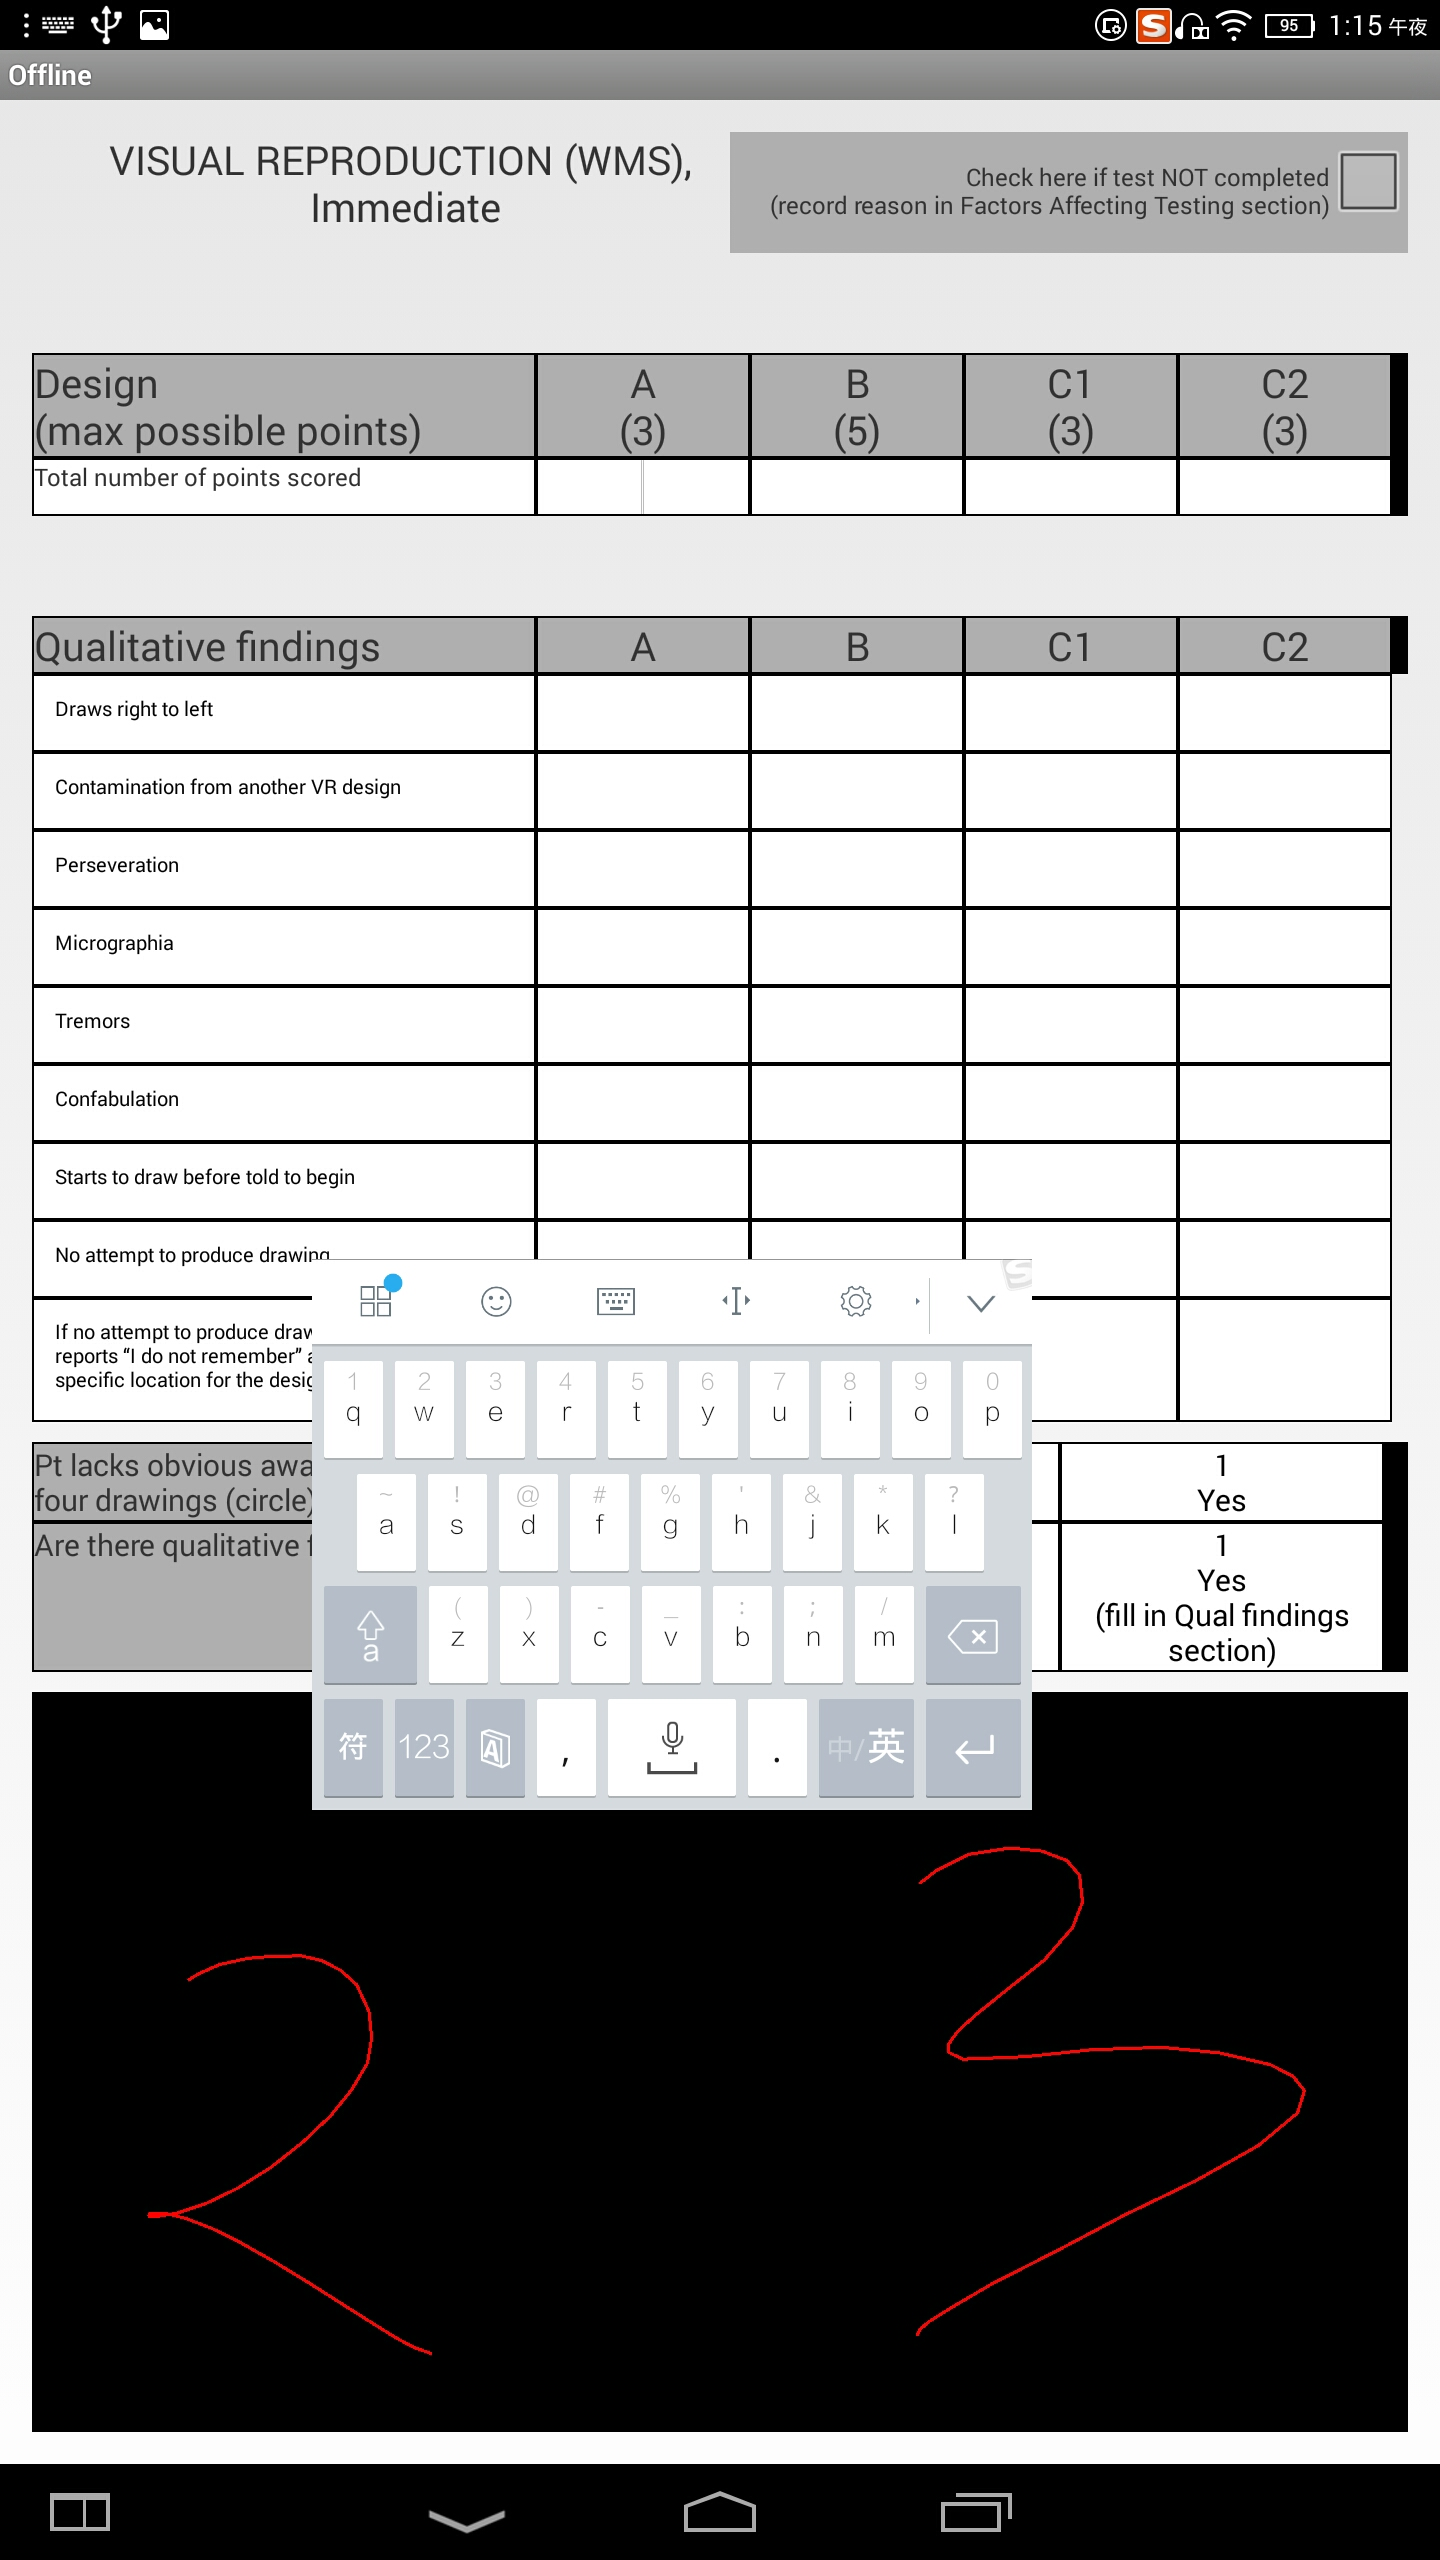
\includegraphics[width=6cm]{drawscore}
\caption{画图题离线打分版-最终实现}
\end{subfigure}
\caption{画图题离线打分版设计和最终实现图}
\label{fig:big1-subfigure}
\end{figure}

离线打分版只需展示各打分选项和图片即可。界面加载时会从OSS平台下载所需资源(用户所画的图)。打分选项的实现与故事复述题离线打分版的打分选项的实现类似,每一个打分选项用自定义的界面组件SingleDrawScoreView表现,统计分数时统计每一个组件的分数并取和。图片的显示运用了ImageView来展示。

\section{单词对复述题模块}

\begin{figure}[h]
\centering%
\includegraphics[width=13cm]{trailA}
\caption{单词对复述题逻辑流程图}
\label{fig:big1-subfigure}
\end{figure}

\begin{figure}[h]
\centering%
\begin{subfigure}{6cm}
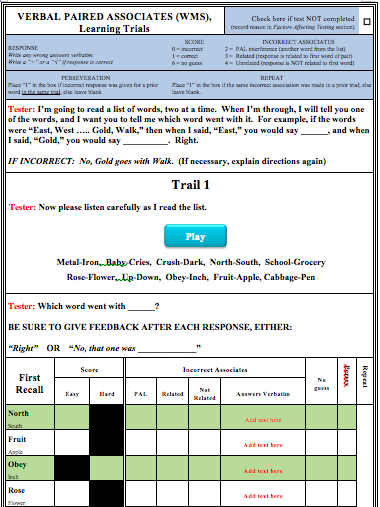
\includegraphics[width=6cm]{trailerD}
\caption{单词对复述复述题-设计}
\end{subfigure}
\hspace{4em}%
\begin{subfigure}{6cm}
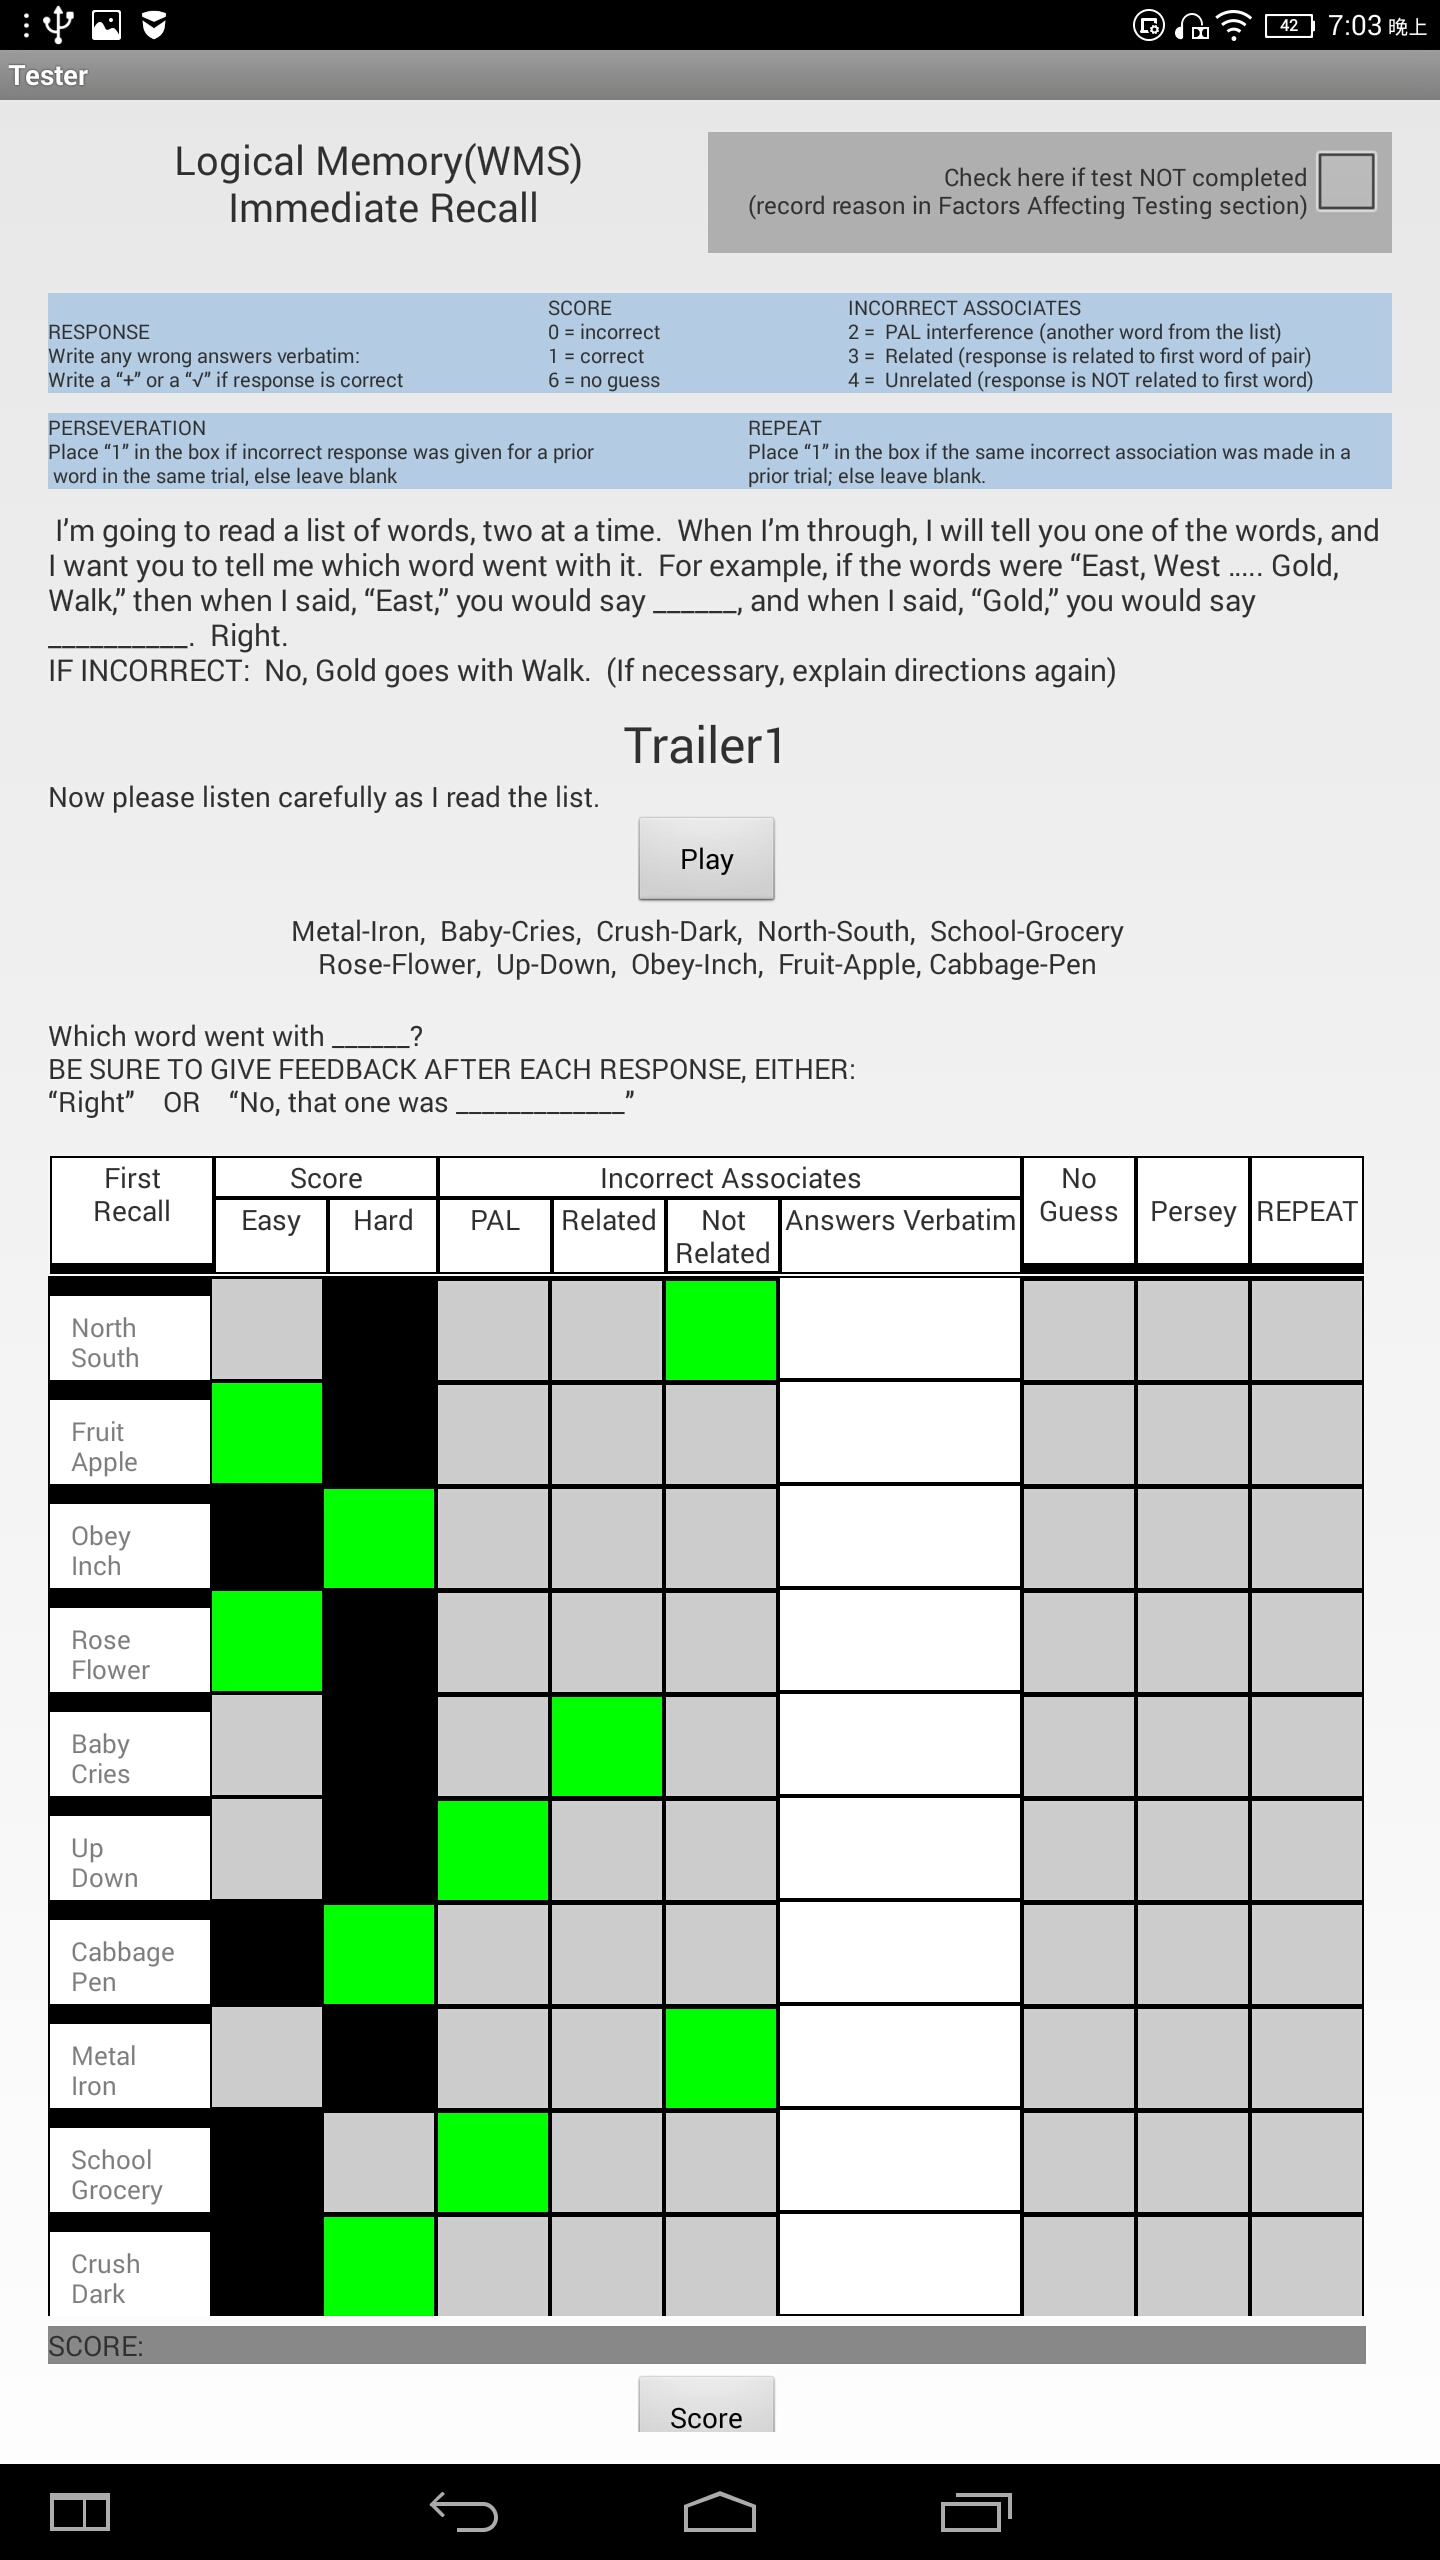
\includegraphics[width=6cm]{trailer}
\caption{单词对复述题-最终实现}
\end{subfigure}
\caption{单词对复述题设计和最终实现图}
\label{fig:big1-subfigure}
\end{figure}

单词对复述题模块的在线测试版和离线打分版一样。这个模块略微复杂,为整个模块设计了对应的界面组件:TrailView和SingleTrailView。其中SingleTrailView只包含一个单词对,而TrailView包含的是一组单词对(TrailActivity包含若干个TrailView,每个TrailView包含若干个SingleTrailView)。一个SingleTrailView包含了一个单词对和其对应的题目显示(包括多个按钮、输入框);TrailView除了包含多个SingleTrailView外还包含一些题目其他信息和获取分数按钮。这样设计是因为每个单词对是相互独立的,SingleTrailView让他们的按钮都能关联起来,TrailView不用管每个单词对的内部逻辑,让结构更简单化。在逻辑中,当Activity启动时,将题目内容更新到其成员TrailView,再让该成员将对应内容更新到TrailView。当用户对题目进行回答时,修改的是SingleTrailView,这时在SingleTrailView中会临时存储用户的答案。获取分数的按钮被设置在TrailView中,当用户点击时会TrailView会从成员SingleTrailView获取到答案信息并更新(但不会告知Activity)。只有当用户在界面上点击“下一页”时,才会从TrailView获取到答案并更新(当然,TrailView会递归地从SingleTrailView获取答案)和上传。

这里为了方便用户的一些操作,设计了“错误字典”,即每个错误的单词会记录下它的错误类型,这样在之后的输入中只要错误单词在字典中,就能很快得得到它的错误类型而不需要再进行错误类型的选择。

单词对复述题分为两种,一种是即时回答,另一种是稍微回答,界面略有不同,模块会根据题目JSON中的信息进行区分并展现不同的界面。


\section{数字串复述题模块}

\begin{figure}[h]
\centering%
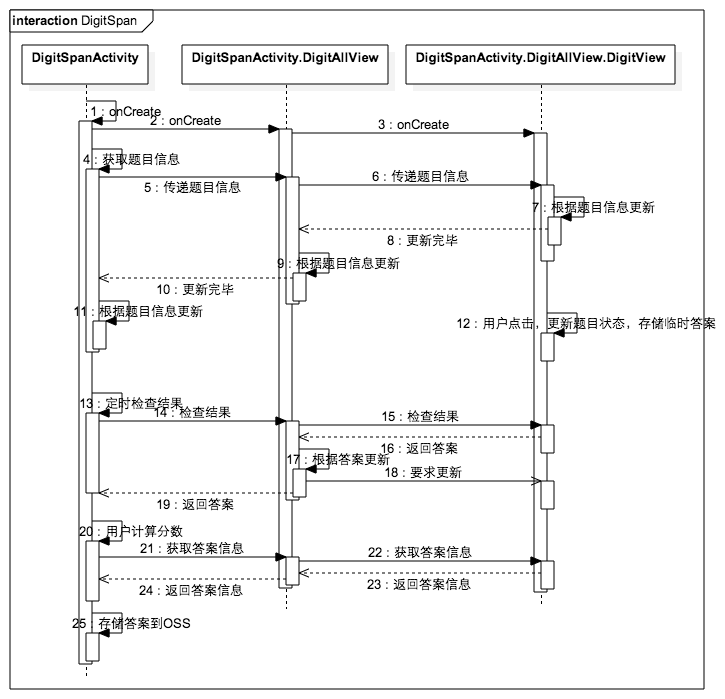
\includegraphics[width=13cm]{DigitSpan}
\caption{数字串复述题逻辑流程图}
\label{fig:big1-subfigure}
\end{figure}

\begin{figure}[h]
\centering%
\begin{subfigure}{6cm}
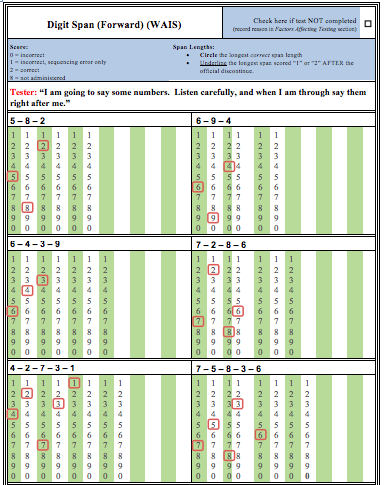
\includegraphics[width=6cm]{digitD}
\caption{数字串复述题-设计}
\end{subfigure}
\hspace{4em}%
\begin{subfigure}{6cm}
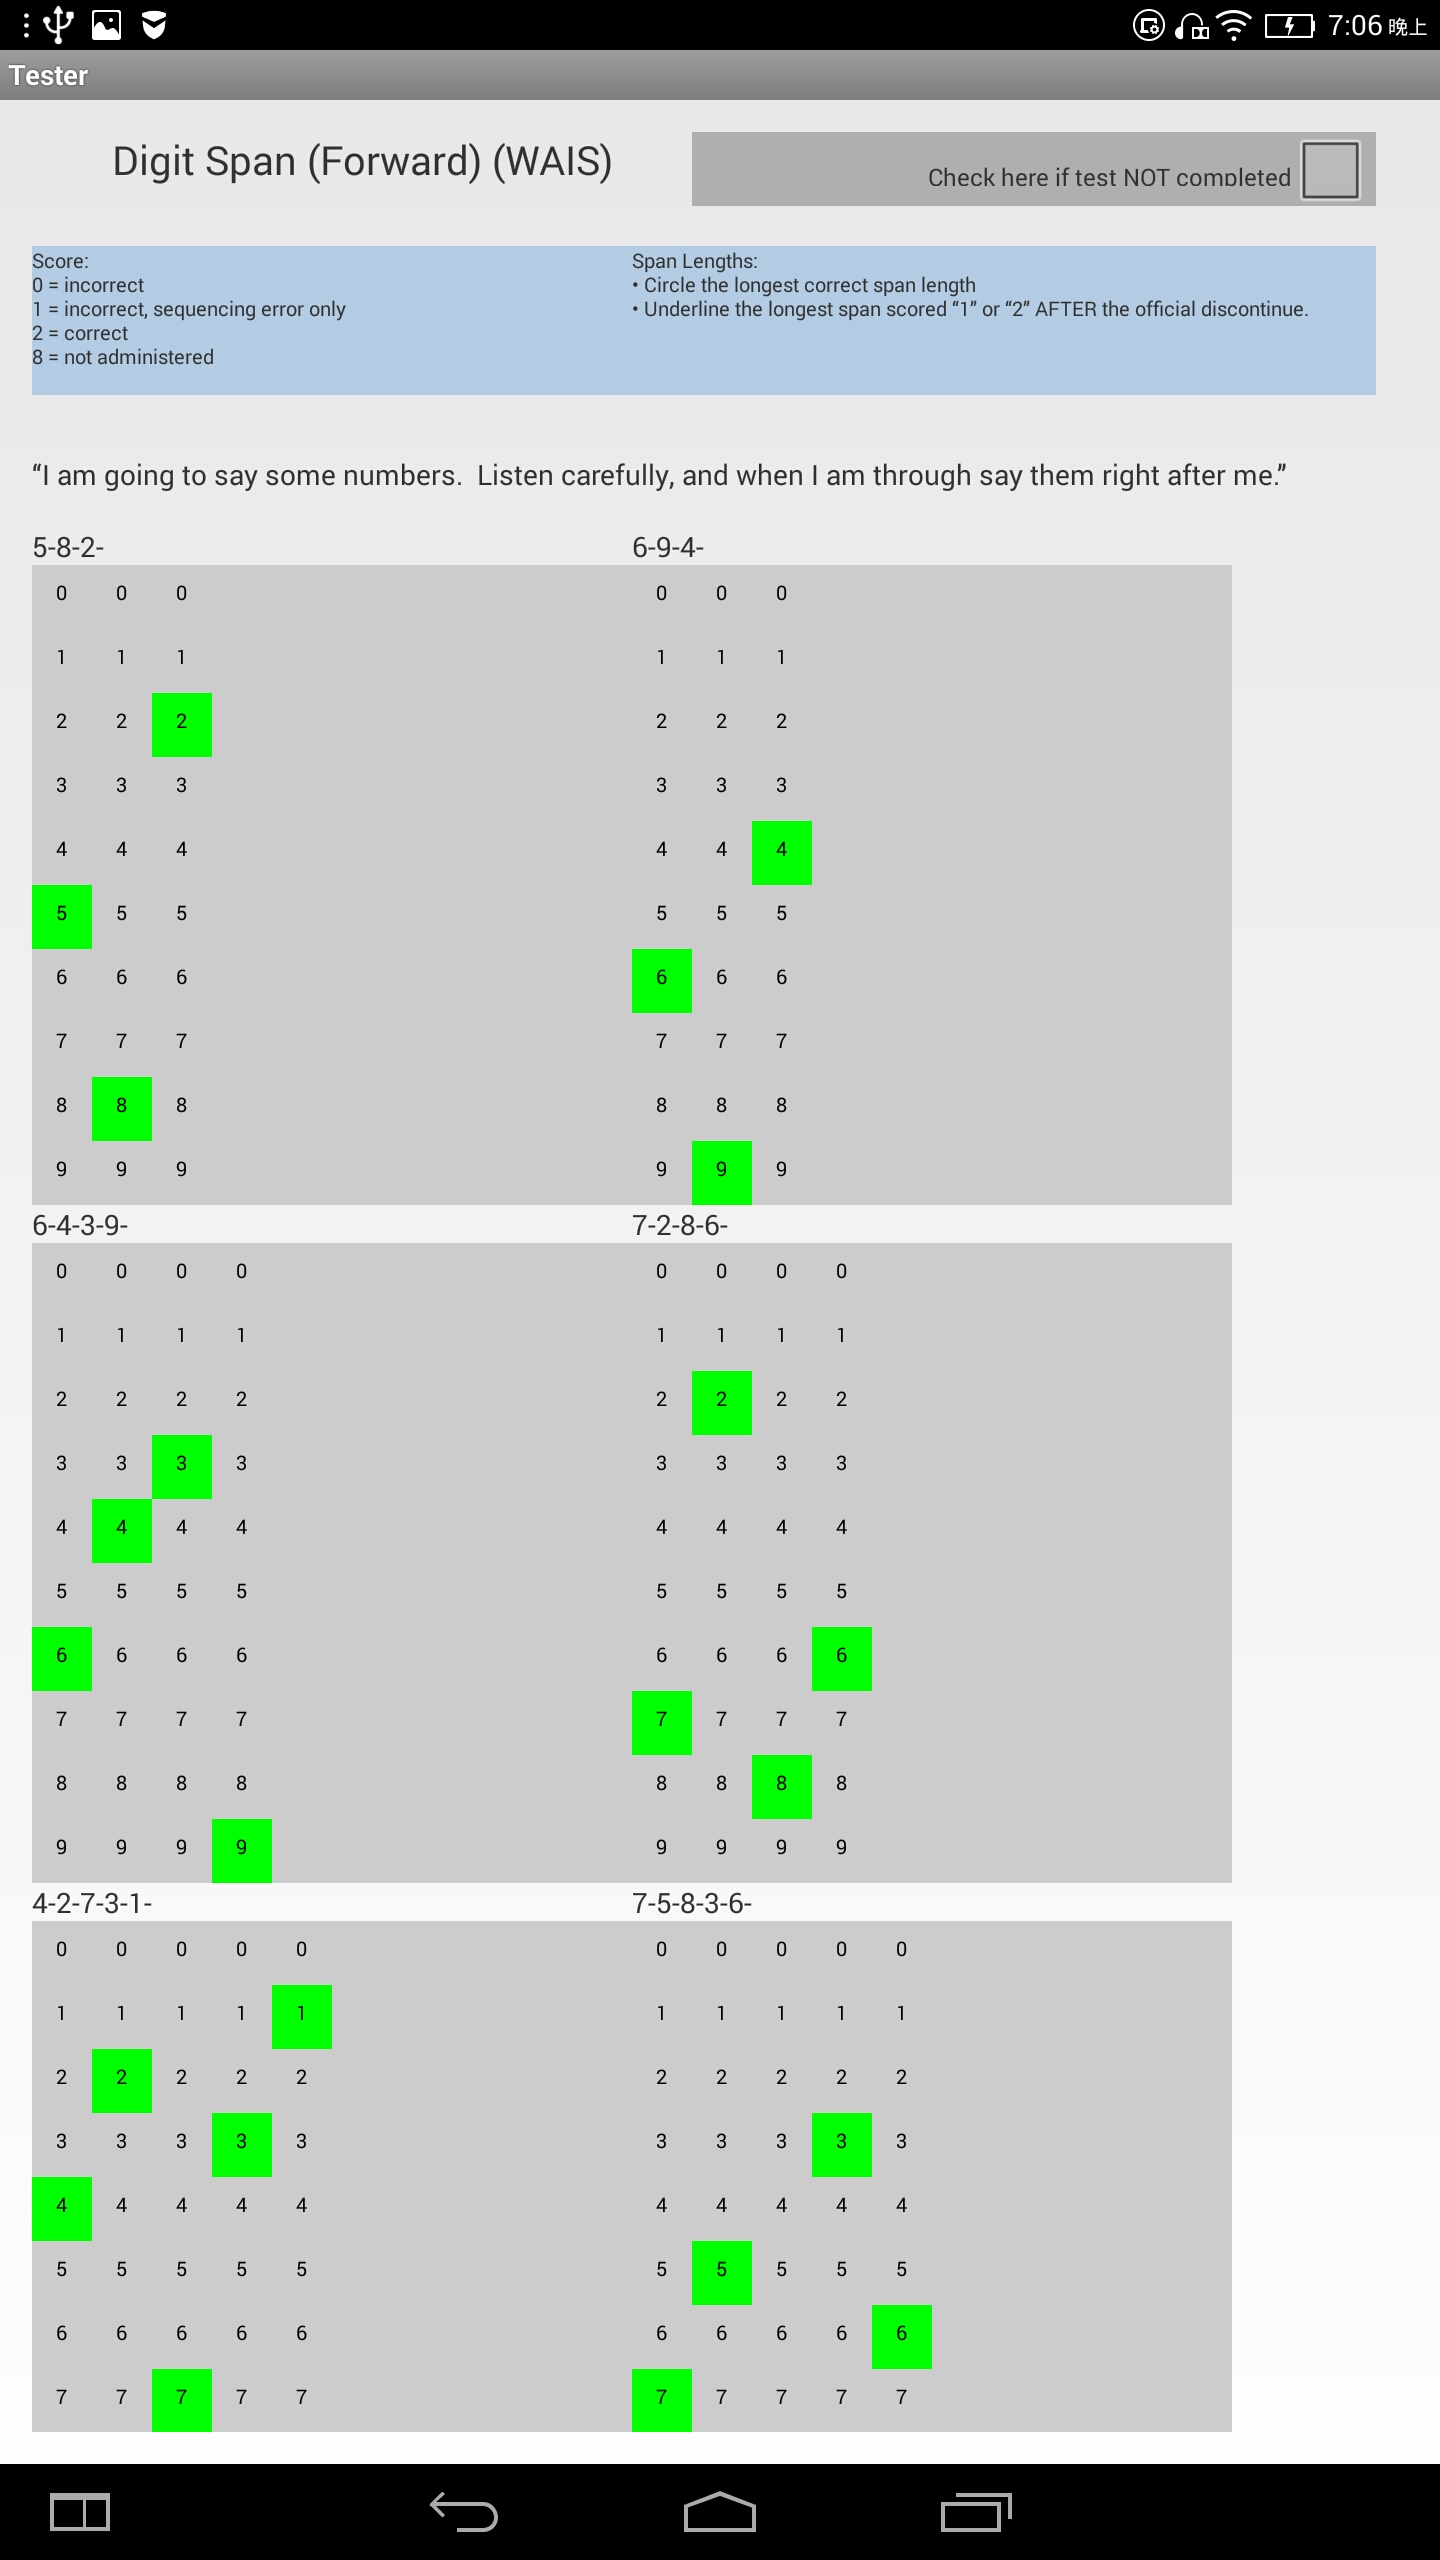
\includegraphics[width=6cm]{digit}
\caption{数字串复述题-最终实现}
\end{subfigure}
\caption{数字串复述题设计和最终实现图}
\label{fig:big1-subfigure}
\end{figure}

数字串复述题模块也相对复杂,与单词对复述题类似,设计了对应的界面组件:DigitAllView和DigitView。DigitView包含了一列可选数字(0-9),而DigitAllView是包含了一道数字串复述的题目。这样的设计思想和单词对复述题的设计思想类似,将独立的部分分开,使系统结构更简单更清晰。当Activity启动时会依次更新DigitAllView和DigitView。DigitView负责实时根据用户的选择更新答案。当用户需要计算分数,或是存储答案,则依次从两个组件中获取答案并更新、上传。

为了做到引导医生使用,模块设计也按照顺序显示题目,即开始只显示第一题,第一题结束后根据结果显示下一题。故在Activity中设置了Handler,以200毫秒更新的频率检查所有的DigitAllView,如果满足条件,则让其开启下一题。

\section{选择题模块}

\begin{figure}[h]
\centering%
\begin{subfigure}{6cm}
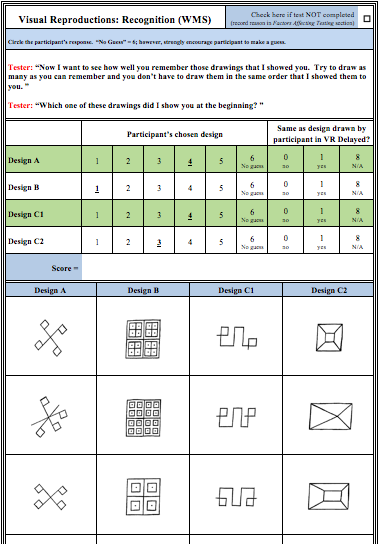
\includegraphics[width=6cm]{choiceD}
\caption{选择题-设计}
\end{subfigure}
\hspace{4em}%
\begin{subfigure}{6cm}
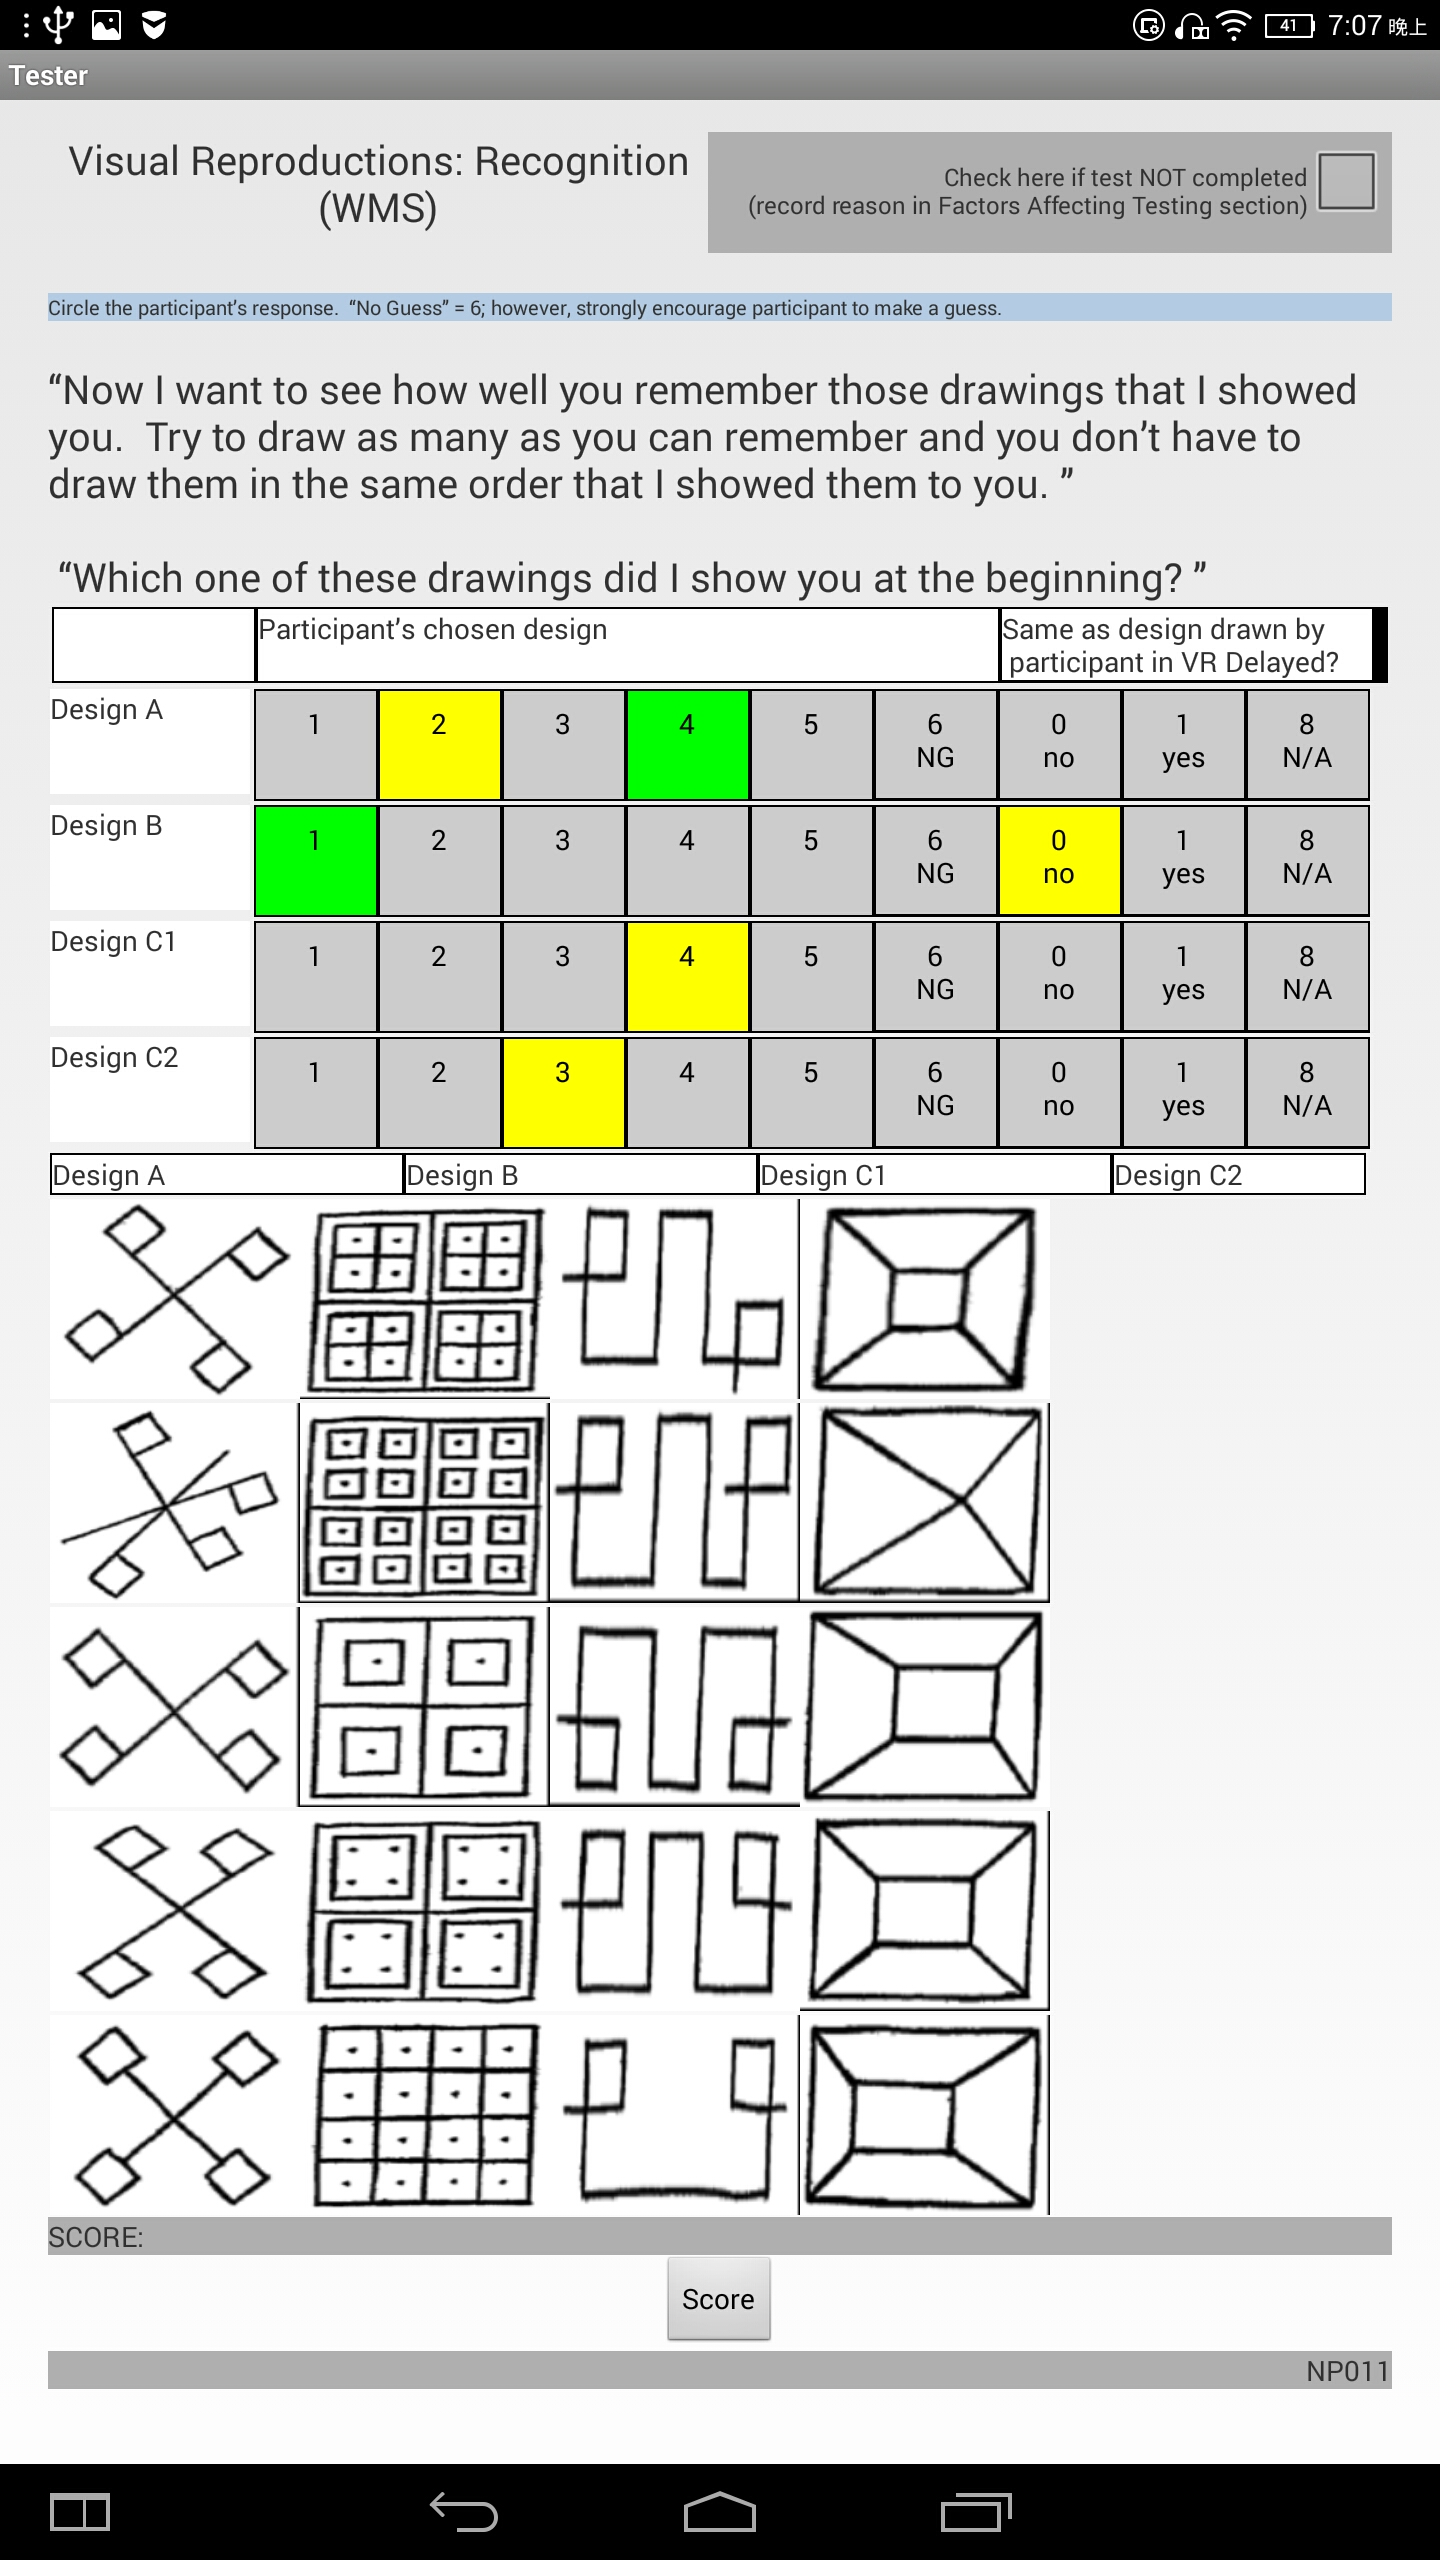
\includegraphics[width=6cm]{choice}
\caption{选择题-最终实现}
\end{subfigure}
\caption{选择题设计和最终实现图}
\label{fig:big1-subfigure}
\end{figure}

为了应对选择题有不同选项、不同表头要求,同样按照数字串复述题和单词对复述题设计了对应界面组件ChoicerView来表示一个选题和其关联的各选项,并临时存储用户选择的答案。当用户需要获取分数时,从每个ChoicerView获取答案并进行统计。当用户需要上传结果时,也从ChoicerView中获取答案并存储。

由于选择题有一种选择画图题,需要另建新图片选择表,在这里直接实现在了Activity里根据对应位置设置了图片按钮,并与对应题目进行关联。临时答案依旧存储在ChoicerView中。


\section{其他模块}

目前设计的其他模块只有结束界面,因为不需要花俏的界面,目前只有显示一行“Finished. Thank you!”的字样。


